\documentclass[12pt,a4paper]{scrartcl}
\usepackage[utf8]{inputenc}
\usepackage[english,russian]{babel}
\usepackage{indentfirst}
\usepackage{misccorr}
\usepackage{graphicx}
\usepackage{amsmath}
\usepackage{multirow}
\usepackage{pgfplots}
\usepackage[top=1cm, bottom=1cm, left=1cm, right=1cm]{geometry}
\pgfplotsset{compat=1.9}

\begin{document}
	\graphicspath{{C:/Users/Alex/OneDrive/Изображения/TexImgs}}
	
	\newcommand{\ms}{\mathstrut}
	\newcommand{\msp}{\hspace{0.5cm}}
	\newcommand{\al}{\alpha}
	\newcommand{\dg}{^\circ}
	\newcommand{\qd}[2]{^{\frac{#1}{#2}}}
	\newcommand{\qdm}[2]{^{-\frac{#1}{#2}}}
	\newcommand{\lm}[2]{\underset{#1 \rightarrow #2}{\lim}}
	\newcommand{\sfrac}[2]{\dfrac{\strut #1}{\strut #2}}
	\newcommand{\equal}[1]{\overset{(#1)}{=}}
	\newcommand{\linevdots}{\ \raisebox{-.08\height}{\vdots}\ }
	\newcommand{\linecvdots}{\ \raisebox{-.08\height}{\vdots}\hspace{-0.13cm}\raisebox{.15\height}{\cancel{\phantom{a}}\hspace{0.06cm}}}
	\newcommand{\combox}[1]{\ms \msp \msp \begin{minipage}{0.95\linewidth}
			#1
	\end{minipage}}
	
	\newtheorem{pr}{Задача}
	\newtheorem{ex}{Пример}
	\newtheorem{dfn}{Def}
	\newtheorem{theorem}{Th}
	\newtheorem{st}{St}
	
	\newenvironment{slv}{\ms \msp \textit{Решение:}}{}
	\newenvironment{proof}{\ms \msp \textit{Доказательство: }}{\hfill $\square$}
	
	\begin{titlepage}
		
		\vspace*{\fill}
		
		\begin{center}
			
\includegraphics[scale=0.8]{MIPT.png}
			\\[0.7cm]\Huge Московский Физико-Технический Институт\\(национальный исследовательский университет)
			\\[2cm]\LARGE Отчет по эксперименту
			\\[0.5cm]\noindent\rule{\textwidth}{1pt}
			\\\Huge\textbf{Измерение моментов инерции твердых тел\\с помощью трифилярного подвеса}
			\\[-0.5cm]\noindent\rule{\textwidth}{1pt}
		\end{center}
		
		\begin{flushleft}
			\textit{Работа №1.2.3; дата: 06.12.21}\hfill\textit{Семестр: 1}
		\end{flushleft}
		
		\vspace*{\fill}
		
		\begin{flushleft}
			Выполнил: \hspace{\fill} Группа:
			\\Кошелев Александр \hspace{\fill} Б05-105
		\end{flushleft}
	\end{titlepage}
	
	%Страница 2
	
	\begin{flushleft}
		\footnotesize{Измерение моментов инерции твердых тел с помощью трифилярного подвеса} \hspace{\fill} \footnotesize{2}
		\\[-0.3cm]\noindent\rule{\textwidth}{0.3pt}
	\end{flushleft}

	\section{Аннотация}
	
	В данной работе рассматривается так называемый трифилярный подвес, который представляет собой подвешенную на трех тросах платформу. При помощи возбуждения и последующего анализа крутильных колебаний этой платформы можно экспериментально определять моменты инерции тел сложной геометрии.
	
	\textbf{Цель работы:}
	Измерение момента инерции ряда тел и сравнение результатов с расчетами по теоретическим формулам; проверка аддитивности моментов инерции и справедливости теоремы Гюйгенса-Штейнера.

	\textbf{В работе используются:} трифилярный подвес, счетчик числа колебаний, набор тел для измерений (толстостенное кольцо, цилиндр из двух половинок, "крышка", брусок).

	\section{Теоретические сведения}
	\begin{dfn}[Момент инерции]
		Моментом инерции тела называется мера его инертности при вращательном движении. Для материальной точки, находящейся на расстоянии $\rho$ от оси вращения $J = m\rho^2$. Соответственно, для протяженного тела формула принимает вид:
		
		$$J = \underset{m}{\int}\rho^2 \mathrm{d}m$$
	\end{dfn}

	Согласно определению, прямым интегрированием можно получить формулы для некоторых из исследуемых тел, приведем их без вывода.
	
	\begin{st}[Моменты инерции некоторых тел] \hfill
		\begin{enumerate}
			\item Толстостенное кольцо с внешним радиусом $R$, внуренним радиусом $r$, массой $m$ относительно оси, проходящей перпендикулярно плоскости кольца через его центр:
			$$J = \sfrac{m(R^2 + r^2)}{2}$$
			
			\item Цилиндр радиуса $R$ и массой $m$ относительно оси, проходящей перпендикулярно плоскости цилиндра через его центр:
			$$J = \sfrac{mR^2}{2}$$
			
			\item Брусок измерениями $w$, $d$, $h$ и массой $m$ относительно оси, проходящей перпендикулярно плоскости измерений $w$ и $d$ через геометрический центр сечения:
			$$J = \sfrac{m(w^2 + d^2)}{12}$$
		\end{enumerate}
	\end{st}

	\newpage
	%Страница 3
	
	\begin{flushleft}
		\footnotesize{Измерение моментов инерции твердых тел с помощью трифилярного подвеса} \hspace{\fill} \footnotesize{3}
		\\[-0.3cm]\noindent\rule{\textwidth}{0.3pt}
	\end{flushleft}

	В ходе работы необходимо проверить теорему Гюйгенса-Штейнера, итак, сформулируем ее.
	
	\begin{theorem}[Гюйгенса-Штейнера]
		Рассмотрим некоторое тело массой $m$. Пусть $O$ - некоторая ось, проходящая через его центр масс, относительно которой тело имеет момент инерции $J_0$. Возьмем некоторую ось $O'$, параллельную оси $O$ и находящуюся на расстоянии $d$ от нее. Тогда момент инерции тела относительно оси $O'$ может быть представлен в виде:
		$$J = J_0 + md^2$$
	\end{theorem}				

	\section{Экспериментальная установка}

	\begin{center}
		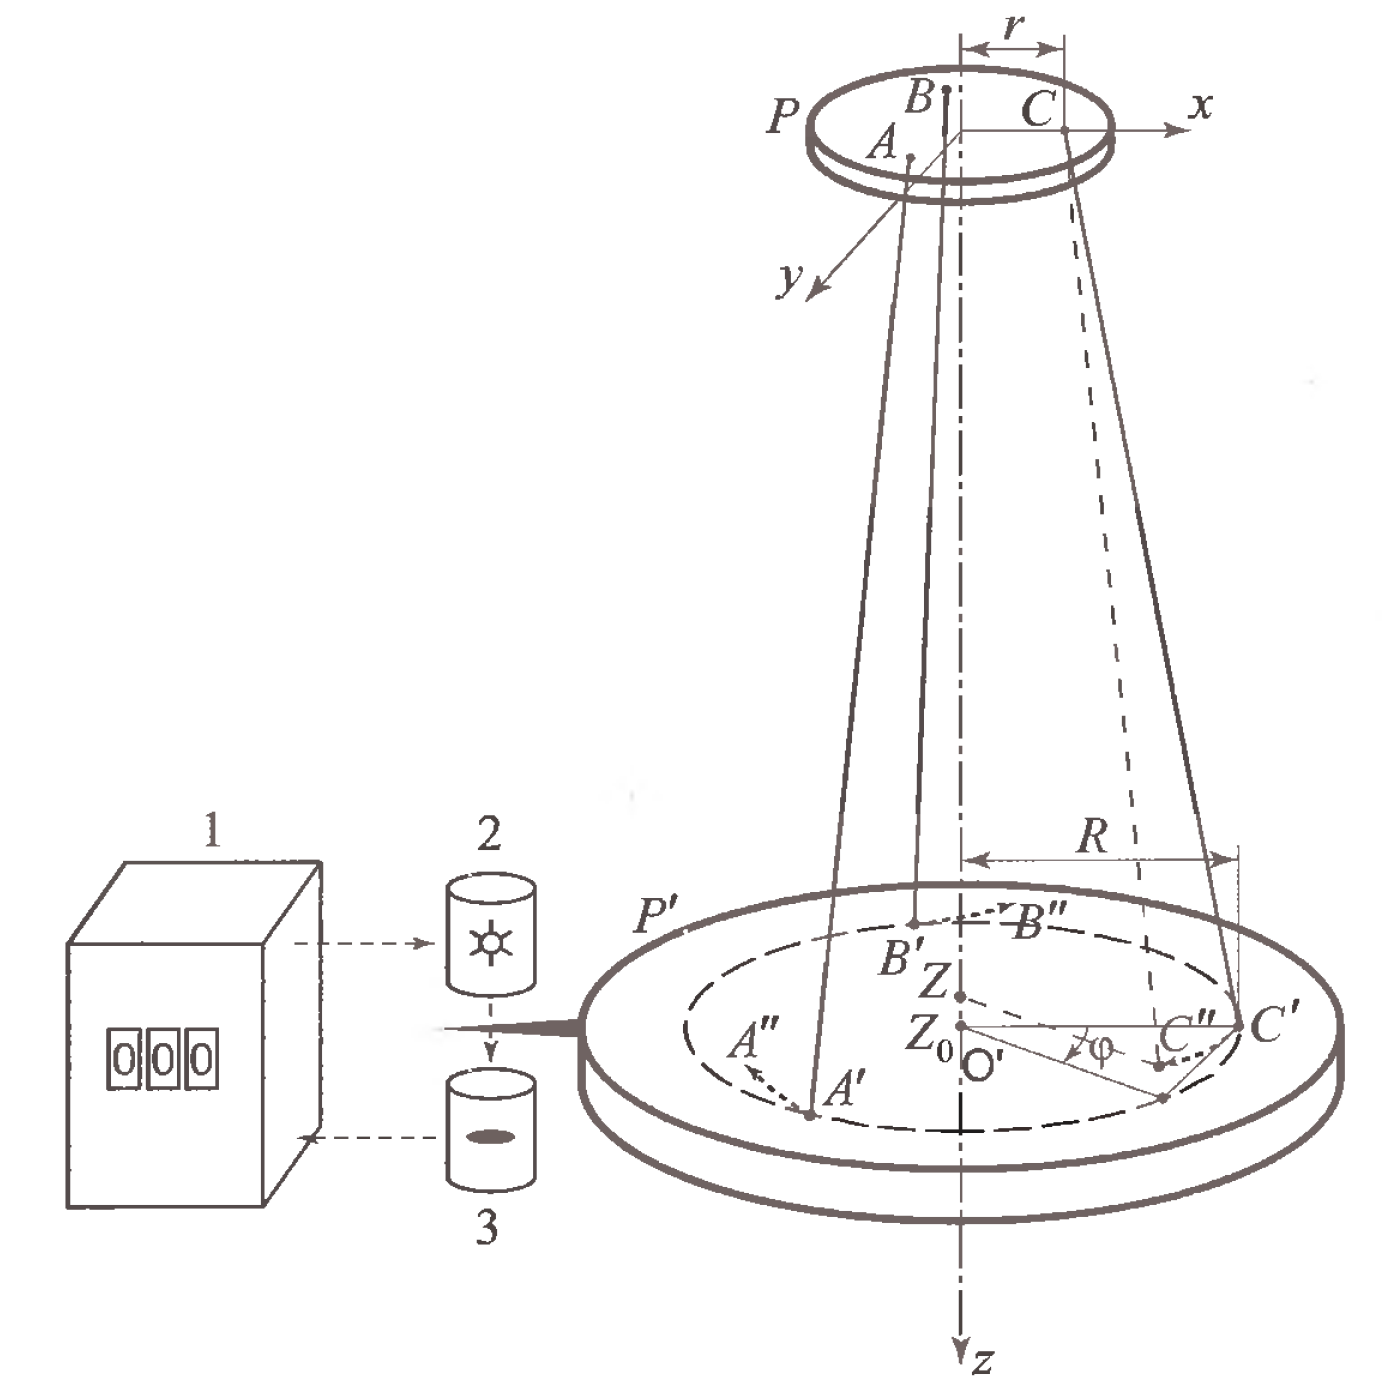
\includegraphics[scale=0.2]{PIC_1.png}
		\\\textbf{Рис. 1: } Трифилярный подвес
	\end{center}

	Данное устройство состоит из укрепленной на некоторой высоте неподвижной платформы $P$, и подвешенной на симметрично расположенных нитях $AA'$, $BB'$ и $CC'$ вращающейся платформы $P'$.
	
	Платформа $P$ снабжена находится на роторе электродвигателя, закрепленного на потолке, при помощи которого можно возбудить крутильные колебания в системе платформ.
	
	После того, как платформа $P$ поворачивается на некоторый угол $\varphi$ (при этом платформа $P'$ приподнимается) в системе возникает вращающий момент, стремящийся вернуть систему в изначальное положение равновесия. При этом можно записать закон сохранения энергии, если пренебречь (малым) трением о воздух:
	
	$$\sfrac{J\overset{\,.}{\varphi}}{2} + mg(z_0 - z) = E = \mathrm{const}$$
	
	Здесь $J$ - момент инерции платформы $P'$ вместе с исследуемым телом, $m$ - масса платформы $P'$ вместе с исследуемым телом, $z_0$ - координата $z$ платформы $P'$ в положении равновесия, $z$ - координата платформы $P'$ при повороте платформы $P$ на угол $\varphi$.
	
	Воспользуемся системой координат, изображенной на рисунке. Координаты точки подвеса одной из нитей $C(r, 0, 0)$. Нижний конец этой нити $C'$ имеет координаты $(R, 0, z_0)$ в положении равновесия, а при повороте $P$ на угол $\varphi$ переходит в $C''$ с координатами $(R\cos \varphi, R\sin \varphi, z)$. Тогда расстояние между точками $C$ и $C''$ равно длине нити $L$:
	
	$$(R\cos \varphi - r)^2 + R^2 \sin^2 \varphi + z^2 = L^2$$
	
	Учтем малость крутильных колебаний, при этом $\cos \varphi \approx 1 - \varphi^2/2$:
	
	$$z^2 = L^2 - R^2 - r^2 + 2Rr\cos \varphi = z_0^2 - 2Rr(1 - cos \varphi) \approx z_0^2 - 2Rr\varphi^2$$
	
	\newpage
	%Страница 4
	
	\begin{flushleft}
		\footnotesize{Измерение моментов инерции твердых тел с помощью трифилярного подвеса} \hspace{\fill} \footnotesize{4}
		\\[-0.3cm]\noindent\rule{\textwidth}{0.3pt}
	\end{flushleft}

	Таким образом:
	
	$$z \approx \sqrt{z_0^2 - 2Rr\varphi} = z_0\sqrt{1 - \sfrac{2Rr\varphi^2}{z_0^2}} \approx z_0 - \sfrac{Rr\varphi^2}{2z_0}$$
	
	Подставим данное значение $z$ в уравнение закона сохранения энергии, продифференцируем по времени и сократим на $\overset{\,.}{\varphi}$. Таким образом и получаем уравнение малых крутильных колебаний нашей системы:
	
	$$\overset{\,..}{\varphi} + \sfrac{mgRr}{Jz_0}\varphi = 0$$
	
	Период этих колебаний, как видно из предыдущего уравнения, равен:
	
	$$T = 2\pi\sqrt{\sfrac{Jz_0}{mgRr}}$$
	
	То есть можно выразить момент инерции через период:
	
	$$J = \sfrac{mgRrT^2}{4\pi^2z_0}$$
	
	Учитывая, что параметры установки в ходе опыта неизменны, можно ввести коэффициент пропорциональности $k = \frac{gRr}{4\pi^2z_0}$, не зависящий от исследуемого тела:
	
	$$J = kmT^2$$

	Таким образом, получена формула для определения момента инерции исследуемого тела вместе с подвижной платформой в допущении малости потерь энергии, что, в сущности означает, что период колебаний $T \ll \tau_{1/2}$ времени полузатухания колебаний.
	
	Для счета числа колебаний используется электронный счетчик, состоящий из оптопары (2-3) и собственно счетчика 1. Лепесток, укрепленный на платформе, дважды за период пресекает луч оптопары, что и регистрирует счетчик.

	
	\section{Проведение эксперимента}
	
	\paragraph{Оценка необходимого времени измерения} \hfill
	\par Проведем измерение с ненагруженной платформой, по нему рассчитаем необходимое время проведения эксперимента, чтобы считать относительную погрешность не превыщающей $0.5\%$.
	
	\begin{center}
		\begin{tabular}{|c|c|c|c|c|c|c|c|c|}
			\hline
			$i$, номер & 1      & 2      & 3      & 4      & 5      & 6      & 7      & 8
			\\\hline
			$20T$, c   & 86.593 & 86.574 & 86.571 & 86.583 & 86.571 & 86.410 & 86.595 & 86.415
			\\\hline
		\end{tabular}
		\\\textbf{Табл. 1: } Пробное измерение
	\end{center}

	Тогда рассчитаем необходимое время измерений:
	$$t = \sfrac{\sigma_t}{\varepsilon_t} \approx 20\ \text{с}$$
	
	\newpage
	
	%Страница 5
	
	\begin{flushleft}
		\footnotesize{Измерение моментов инерции твердых тел с помощью трифилярного подвеса} \hspace{\fill} \footnotesize{5}
		\\[-0.3cm]\noindent\rule{\textwidth}{0.3pt}
	\end{flushleft}

	\paragraph{Измерение времени затухания колебаний} \hfill
	\par Измерим время затухания амплитуды колебаний в два раза. Точное время определить проблематично, поэтому приведем приблизительное значение:
	
	$$\tau_{1/2} \approx 320\ \text{с}$$
	
	Таким образом, полученные формулы действительно справедливы, так как все периоды окажутся много меньше.
	
	\paragraph{Диапазон амплитуд колебаний} \hfill
	\par Рабочий диапазон амплитуд колебаний напрямую определяется областью применимости теоретических формул. Приблизительное значение $\varphi_{max} = 10^\circ$.
	
	\paragraph{Экспериментальное измерение моментов инерции тел} \hfill
	\par Вначале составим таблицу параметров системы и вычислим необходимый коэффициент $k$.
	
	\begin{center}
		\begin{tabular}{|c|c|c|c|c|}
			\hline
			$R$, мм & $r$, мм & $m$, г & $z_0$, м & $k$, м$^2$/с$^2$
			\\\hline
			$114.6 \pm 0.5$ & $30.5 \pm 0.3$ & $1012.5 \pm 0.5$ & $2.152 \pm 0.005$ & $(4.03 \pm 0.18)\cdot10^{-4}$
			\\\hline
		\end{tabular}
		\\\textbf{Табл. 2: Параметры подвеса}
	\end{center}

	\paragraph{Пустая платформа} \hfill
	
	\par Для пустой платформы запишем таблицу измерений:
	
	\begin{center}
		\begin{tabular}{|c|c|c|}
			\hline
			$i$ & $T$, с & $m$, г
			\\\hline
			1 & $4.330 \pm 0.004$ & \multirow{8}{*}{$1012.5 \pm 0.5$}
			\\\cline{1-2}
			2 & $4.329 \pm 0.004$ &
			\\\cline{1-2}
			3 & $4.329 \pm 0.004$ &
			\\\cline{1-2}
			4 & $4.329 \pm 0.004$ &
			\\\cline{1-2}
			5 & $4.329 \pm 0.004$ &
			\\\cline{1-2}
			6 & $4.321 \pm 0.004$ &
			\\\cline{1-2}
			7 & $4.330 \pm 0.004$ &
			\\\cline{1-2}
			8 & $4.321 \pm 0.004$ &
			\\\hline
		\end{tabular}
		\\\textbf{Табл. 3: Измерение пустой платформы}
	\end{center}

	Тогда усредним период и рассчитаем момент инерции:
	$$T = 4.327 \pm 0.004\ \text{с}$$
	
	$$J_0 = (7.64 \pm 0.34) \cdot 10^{-3}\ \text{кг}\cdot\text{м}^2$$
	
	\paragraph{Толстостенное кольцо} \hfill
	
	Для толстостенного кольца запишем таблицу измерений:
	
	\begin{center}
		\begin{tabular}{|c|c|c|c|c|c|}
			\hline
			$T$, с & $R$, мм & $r$, мм & $m$, г & $m_{\Sigma}$, г & $J_\Sigma$, $\text{кг}\cdot\text{м}^2$
			\\\hline
			$4.112 \pm 0.021$ & $81.0 \pm 0.1$ & $74.5 \pm 0.2$ & $1049.8 \pm 0.1$ & $2262.3 \pm 0.6$ & $(1.41 \pm 0.06) \cdot 10^{-2}$
			\\\hline
		\end{tabular}
		\\\textbf{Табл. 4: Измерение толстостенного кольца}
	\end{center}

	Таким образом, получаем:
	$$J_{\text{к}} = J_{\Sigma} - J_0 = (6.46 \pm 0.72) \cdot 10^{-3}\ \text{кг}\cdot\text{м}^2$$
	
	Данное значение отлично совпадает с теоретическим значением момента инерции:
	$$\tilde{J}_{\text{к}} = (6.36 \pm 0.01) \cdot 10^{-3}\ \text{кг}\cdot\text{м}^2$$
	
	Этот факт \textbf{подтверждает аддитивность моментов инерции}.
	
	\newpage
	
	%Страница 6
	
	\begin{flushleft}
		\footnotesize{Измерение моментов инерции твердых тел с помощью трифилярного подвеса} \hspace{\fill} \footnotesize{6}
		\\[-0.3cm]\noindent\rule{\textwidth}{0.3pt}
	\end{flushleft}
	
	\paragraph{Цилиндр (из половинок)} \hfill
	
	Для цилиндра запишем таблицу измерений:
	
	\begin{center}
		\begin{tabular}{|c|c|c|c|}
			\hline
			$T$, с & $m$, г & $m_{\Sigma}$, г & $J_\Sigma$, $\text{кг}\cdot\text{м}^2$
			\\\hline
			$3.082 \pm 0.015$ & $1416.7 \pm 0.1$ & $2429.2 \pm 0.6$ & $(9.32 \pm 0.43) \cdot 10^{-3}$
			\\\hline
		\end{tabular}
		\\\textbf{Табл. 5: Измерение цилиндра}
	\end{center}

	Тогда:
	
	$$J_{\text{цил}} = J_\Sigma - J_0 = (2.96 \pm 0.55) \cdot 10^{-3}\ \text{кг}\cdot\text{м}^2$$
	
	\paragraph{Крышка} \hfill
	
	Для крышки запишем таблицу измерений:
	
	\begin{center}
		\begin{tabular}{|c|c|c|c|}
			\hline
			$T$, с & $m$, г & $m_{\Sigma}$, г & $J_\Sigma$, $\text{кг}\cdot\text{м}^2$
			\\\hline
			$3.892 \pm 0.019$ & $589.6 \pm 0.1$ & $1602.1 \pm 0.6$ & $(9.81 \pm 0.45) \cdot 10^{-3}$
			\\\hline
		\end{tabular}
		\\\textbf{Табл. 6: Измерение крышки}
	\end{center}
	
	Тогда:
	
	$$J_{\text{кр}} = J_\Sigma - J_0 = (2.17 \pm 0.56) \cdot 10^{-3}\ \text{кг}\cdot\text{м}^2$$
	
	\paragraph{Брусок} \hfill
	
	Для бруска запишем таблицу измерений:
	
	\begin{center}
		\begin{tabular}{|c|c|c|c|}
			\hline
			$T$, с & $m$, г & $m_{\Sigma}$, г & $J_\Sigma$, $\text{кг}\cdot\text{м}^2$
			\\\hline
			$3.688 \pm 0.018$ & $1206.1 \pm 0.1$ & $2218.6 \pm 0.6$ & $(1.22 \pm 0.05) \cdot 10^{-2}$
			\\\hline
		\end{tabular}
		\\\textbf{Табл. 7: Измерение бруска}
	\end{center}
	
	Тогда:
	
	$$J_{\text{бр}} = J_\Sigma - J_0 = (4.56 \pm 0.60) \cdot 10^{-3}\ \text{кг}\cdot\text{м}^2$$
	
	\paragraph{Проверка теоремы Гюйгенса-Штейнера} \hfill
	
	Для проверки воспользуемся разрезанным пополам цилиндром. Будем раздвигать половинки и измерять соответствующие моменты инерции. Построим график зависимости $J(h^2)$. То есть, зависимость должна быть линейной с коэффициентом, равным массе цилиндра.
	
	\begin{center}
		\begin{tabular}{|c|c|c|}
			\hline
			$h$, мм & $T$, с & $J_\Sigma \cdot 10^3$, $\text{кг}\cdot\text{м}^2$
			\\\hline
			0  & $3.080 \pm 0.001$ & $9.31 \pm 0.41$
			\\\hline
			5  & $3.091 \pm 0.001$ & $9.37 \pm 0.42$
			\\\hline
			10 & $3.105 \pm 0.001$ & $9.46 \pm 0.42$
			\\\hline
			15 & $3.129 \pm 0.001$ & $9.61 \pm 0.43$
			\\\hline
			20 & $3.174 \pm 0.001$ & $9.88 \pm 0.44$
			\\\hline
			25 & $3.214 \pm 0.001$ & $10.13 \pm 0.45$
			\\\hline
			30 & $3.286 \pm 0.001$ & $10.60 \pm 0.47$
			\\\hline
			35 & $3.346 \pm 0.001$ & $10.99 \pm 0.49$
			\\\hline
			40 & $3.428 \pm 0.001$ & $11.52 \pm 0.51$
			\\\hline
			45 & $3.509 \pm 0.001$ & $12.08 \pm 0.54$
			\\\hline
			50 & $3.606 \pm 0.001$ & $12.76 \pm 0.57$
			\\\hline
		\end{tabular}
		\\\textbf{Табл. 8: } Построение графика $J_{\Sigma}(h^2)$
	\end{center}
	
	\newpage
	
	%Страница 7
	
	\begin{flushleft}
		\footnotesize{Измерение моментов инерции твердых тел с помощью трифилярного подвеса} \hspace{\fill} \footnotesize{7}
		\\[-0.3cm]\noindent\rule{\textwidth}{0.3pt}
	\end{flushleft}
	
	\begin{center}
		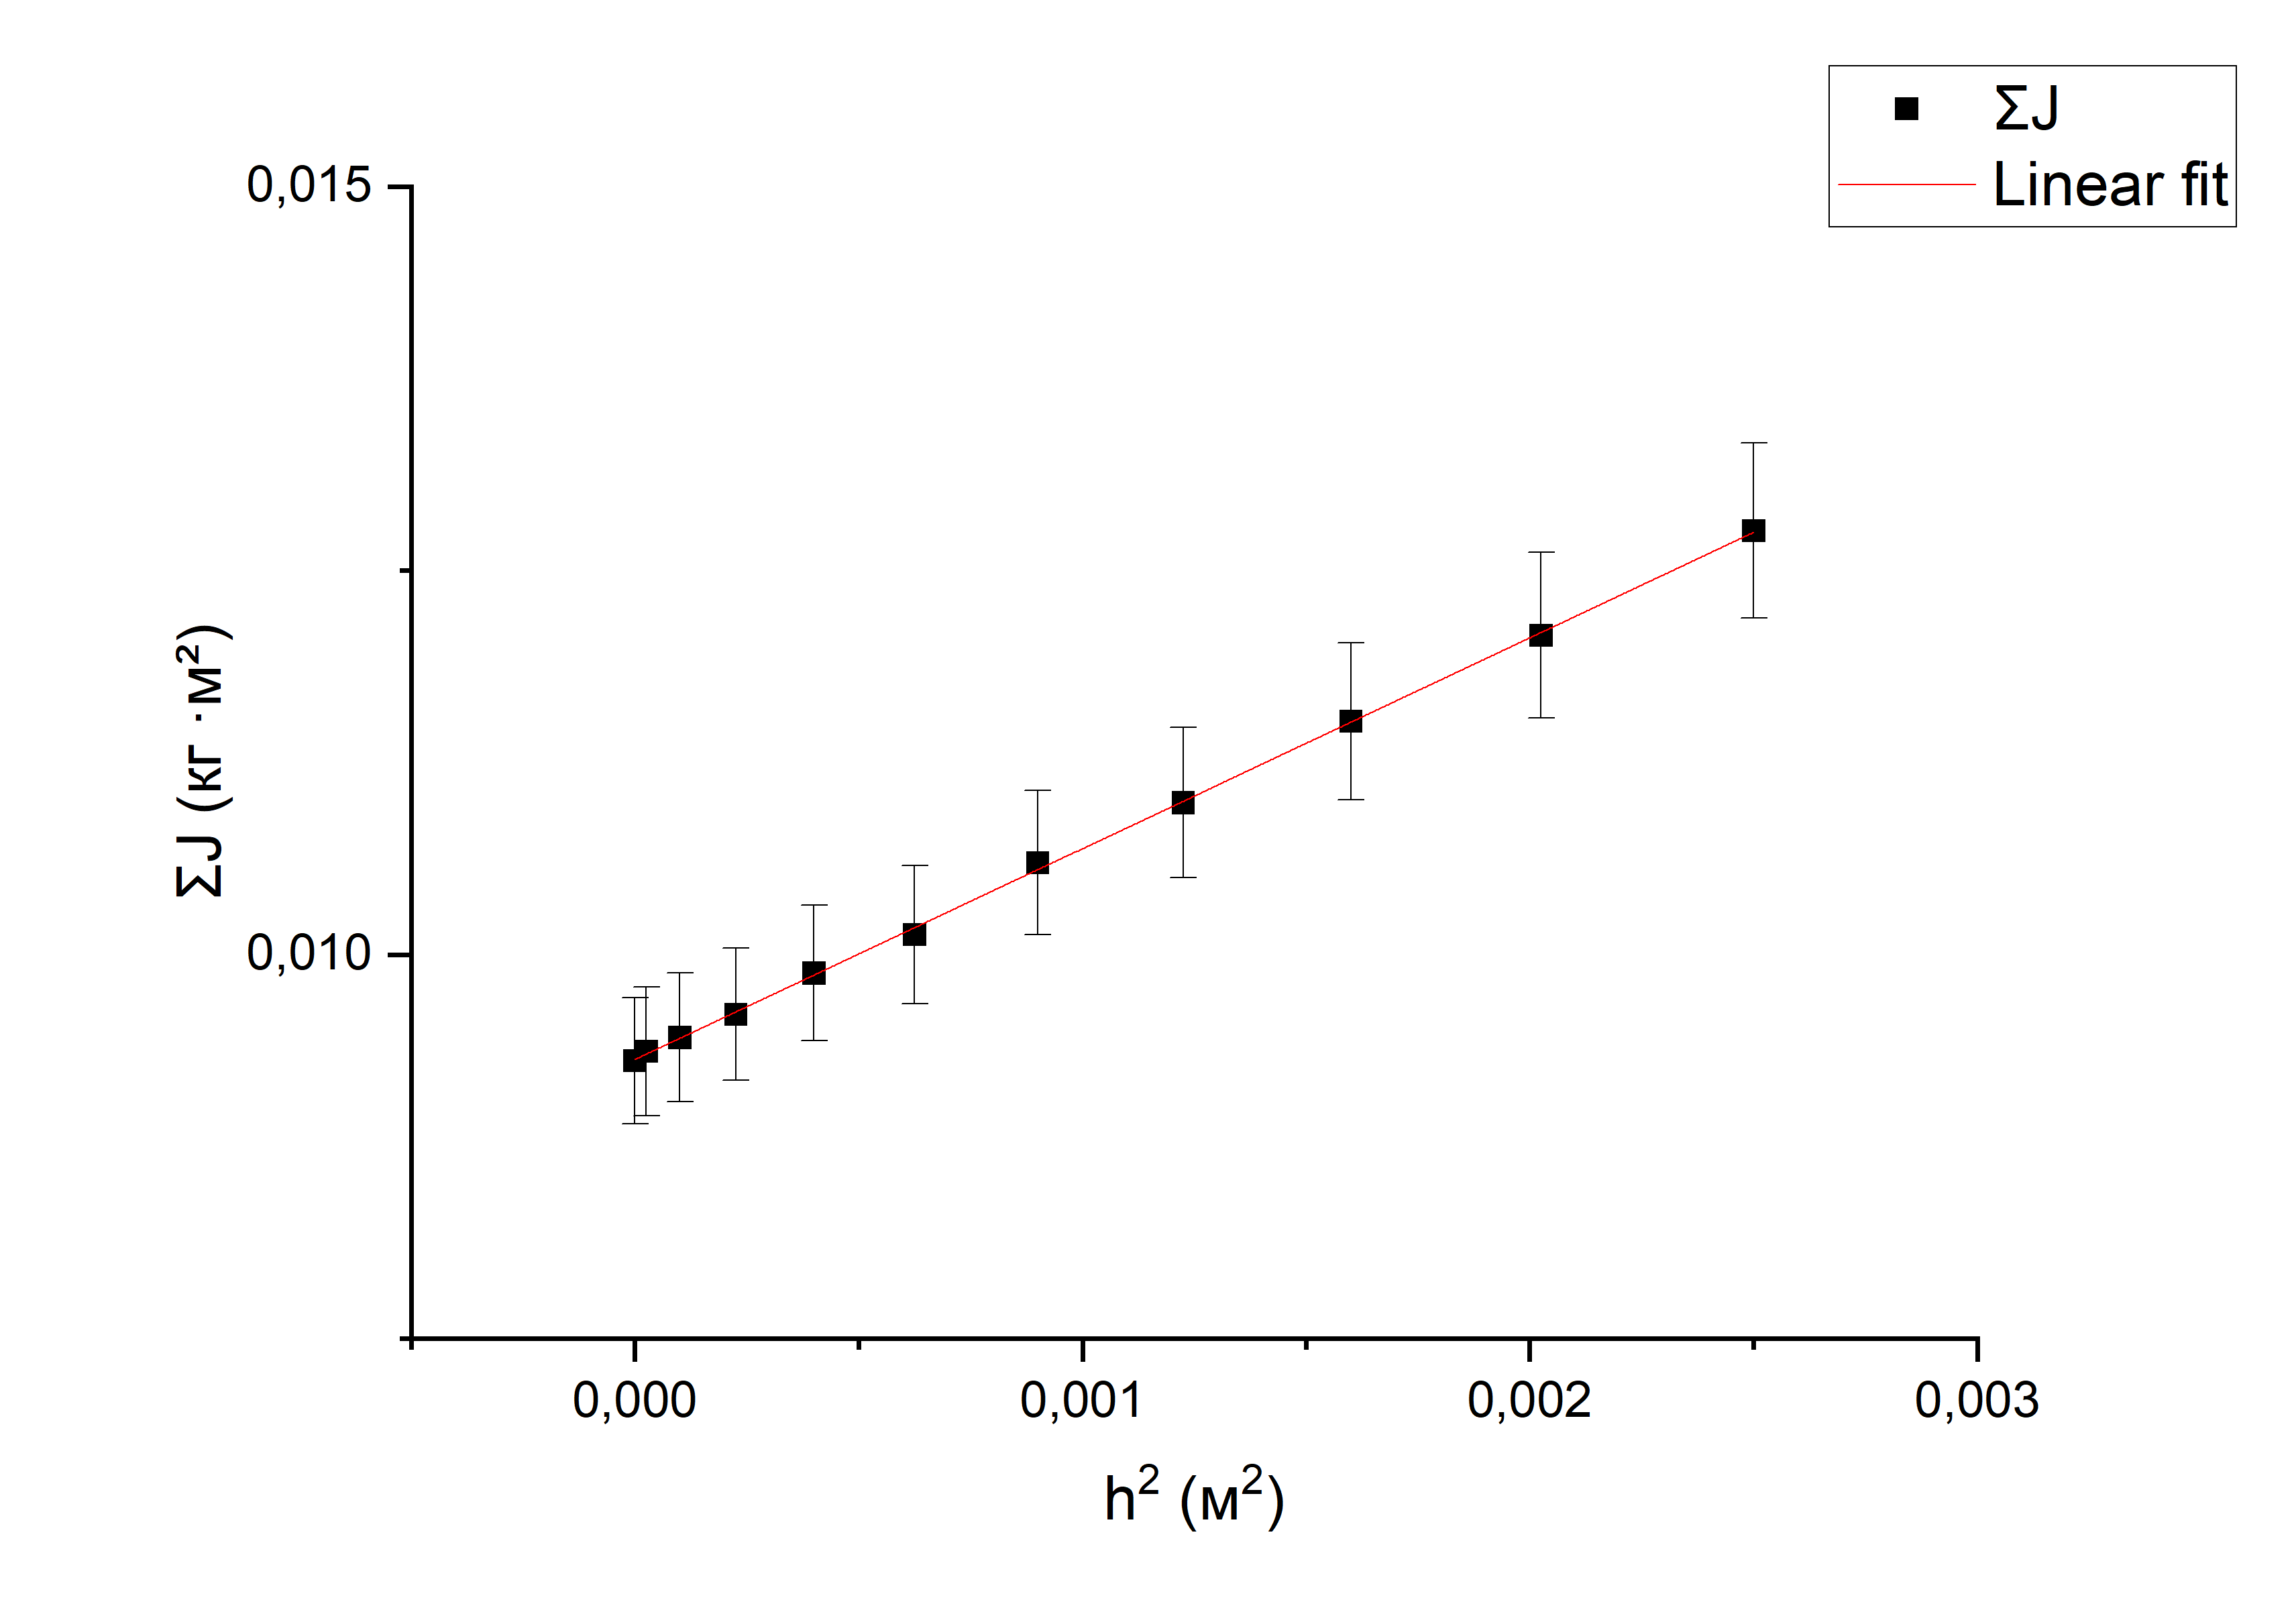
\includegraphics[scale=0.5]{PIC_2.png}
		\\\textbf{Рис. 2: } График зависимости $J(h^2)$
	\end{center}

	Итак, график подтверждает наш вывод о характере данной зависимости. Через МНК получим значение коэффициента наклона и значение в нуле:
	
	$$k_J = 1.373 \pm 0.100\ \text{кг}$$
	$$J_{0\,\Sigma} = (9.32 \pm 0.01) \cdot 10^{-3} \cdot 10^{-3}\ \text{кг}\cdot\text{м}^2$$
	
	Таким образом, данные коэффициенты подтверждают теорему Гюйгенса-Штейнера, так как $k_J$ совпадает с массой цилиндра в пределах половины стандартного отклонения, а $J_{0\,\Sigma}$ совпадает с суммарным моментом инерции платформы и цилиндра в пределах стандартного отклонения.
	
	\section{Выводы}
	В работе произведено измерение моментов инерции ряда тел:
	\begin{enumerate}
		\item Толстостенное кольцо $J_{\text{к}} = (6.46 \pm 0.72) \cdot 10^{-3}\ \text{кг}\cdot\text{м}^2$
		
		\item Цилиндр (из половинок) $J_{\text{цил}} = (2.96 \pm 0.55) \cdot 10^{-3}\ \text{кг}\cdot\text{м}^2$
		
		\item Крышка $J_{\text{кр}} = (2.17 \pm 0.56) \cdot 10^{-3}\ \text{кг}\cdot\text{м}^2$
		
		\item Брусок $J_{\text{бр}} = (4.56 \pm 0.60) \cdot 10^{-3}\ \text{кг}\cdot\text{м}^2$
	\end{enumerate}
	
	На примере кольца результат сверен с теоретической оценкой, полученной путем вывода формулы прямым интегрированием. Результаты совпадают с точностью значительно меньшей величины стандартного отклонения, поэтому считаю результаты удовлетворительными.
	
	Также это значение для кольца подтверждает аддитивность моментов инерции, поскольку значение момента инерии кольца получено именно в допущении, что моменты инерции аддитивны.
	
	Отдельно выделим экспериментальное подверждение теоремы Гюйгенса-Штейнера, которое также получено с весьма хорошей точностью.
	
\end{document}